\chapter{Background}
\label{cha:bg}

Text.


\section{Video compression concepts}
\label{sec:bg/compression}

Video is known to be one of the heaviest types of content to be stored and transmitted. Since treating uncompressed video is unfeasible, video compression or video coding formats have been developed and standardized over the years, with multiple implementations (\textit{codecs}) being released. The objective of video codecs is to limit the output data rate, measured in bits per second, while trying to maintain a perceptually good video quality.

The process of compressing a video is known as \textbf{encoding} and is performed by an encoder. When a video file is already encoded in a video format and needs to be encoded in another one, we often use the term \textbf{transcoding}.

In this section we will go through the main techniques that are used by most video coding standards.

\subsection{RGB vs Y'CbCr}
\label{sec:bg/compression/ycbcr}

The most basic form of compression can be obtained by converting individual pictures representing the video to a \textbf{color space} that better exploits human vision characteristics and then applying compression of some of the components in the new color space.

A very common color space family used in digital video and images is \textbf{Y'CbCr}, sometimes improperly called YUV (which relates to the analog domain), which exploits the fact that the human vision system is much more sensitive to light variations (brightness) than to color. The Y'CbCr color space decomposes the color information of a pixel into three components:

\begin{itemize}
    \item \textbf{Y'}: the luminance, representing the brightness of the image;
    \item \textbf{Cb}: the blue chroma component, representing a projection of the blue color;
    \item \textbf{Cr}: the red chroma component, representing a projection of the red color.
\end{itemize}

This approach is different from the common RGB (Red Green Blue) color space, where the luminance is not isolated from the color components, and allows to apply compression in a more effective way through the \textbf{chroma subsampling} technique.

Chrome subsampling refers to the practice of reducing the resolution of the chroma components while keeping the luminance at full resolution. Since our eyes are less sensitive to color than to brightness, we can reduce the color resolution by even 75\% with almost no perceptual impact on quality.

% sources from LT

The vast majority of digital video that can be found on the Internet or that is transmitted through digital television is compressed with the Y'CbCr 4:2:0 color space, the most common format for non-professional content. In Y'CbCr 4:2:0, the luminance component (Y) is encoded at full resolution, while the chroma components are stored at 1/4 of the resolution, i.e. instead of storing 8 chroma samples for every 8 pixels we only keep 2, as shown in Figure X.

% figure from LT

When compared to a typical 8-bit RGB image (equivalent to Y'CbCr 4:4:4, i.e. no subsampling), requiring 24 bits per pixel, a Y'CbCr 4:2:0 image requires only 12 bits per pixel, resulting in a 50\% saving with very similar perceived quality. When using tools like \texttt{ffmpeg}, Y'CbCr 4:2:0 is often called \texttt{yuv420p} or similar.

\subsection{Inter-frame and intra-frame compression}
\label{sec:bg/compression/intra-inter}

The major video coding standards released since the early 1990s are based on a \textbf{hybrid codec model} that exploits both temporal and spatial redundancy of videos to achieve high compression ratios.

Temporal compression, or \textbf{inter-frame compression}, relies on the fact that there is usually a high similarity between consecutive video frames. On the other hand spatial compression, or \textbf{intra-frame compression}, exploits the fact that pixels that are close to each other within a picture are usually highly correlated.

Video codecs (en\textbf{co}der/\textbf{dec}oder) are implementations of video coding standards that are able to convert the input video into a coded version in a way that is reversible, i.e. such that the decoder can reconstruct the original video with some approximation. Encoders should output a compressed representation that is as efficient as possible while trying to preserve the fidelity of the original video.

\begin{figure}[h]
	\centering
	
	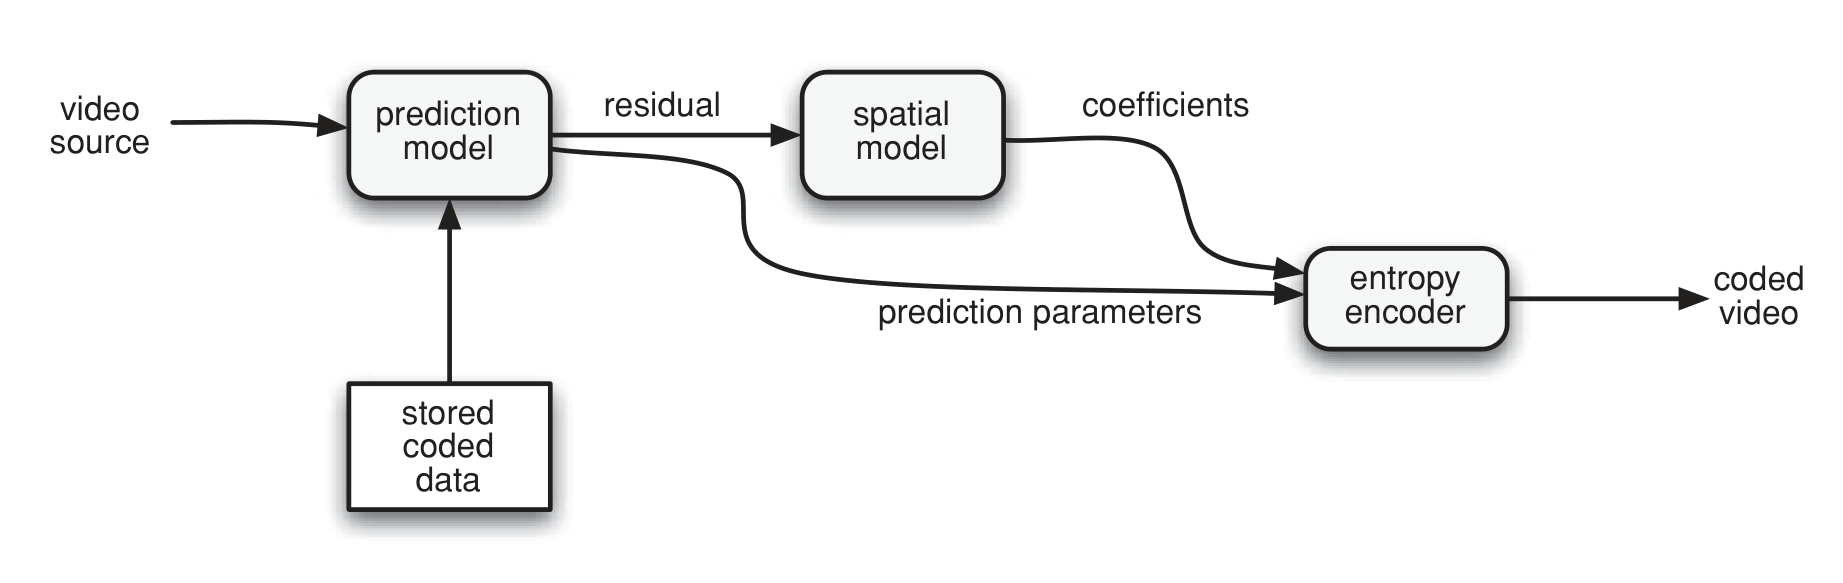
\includegraphics[width=\textwidth]{res/hybrid_codec_high_level.png}
	
	\caption{High-level hybrid codec architecture.\cite{h264}}
	\label{fig:codec_highlevel}
\end{figure}

In general, a hybrid video codec works in three phases:\cite{h264}

\begin{itemize}
    \item \textbf{Prediction model}: exploits spatial or temporal redundancy by producing a prediction of the current frame (or block of a frame) being analyzed, by looking at a previous reference frame or at other parts of the same frame. The outputs of this phase are a \textbf{residual frame}, which is the difference between the actual frame and the predicted frame, and the parameters that define how the prediction was obtained. By encoding only the residual and the parameters we can basically store only the "error" of the prediction and greatly reduce the amount of data that needs to be coded. The prediction can be obtained in two ways:
        \begin{itemize}
            \item \textbf{Temporal prediction}: in its most basic form, the prediction is the difference between the current frame and a previous (or future) reference frame. In practice, we also need to take into account the motion that occurs between frames by running a \textbf{motion estimation} algorithm that for each block\footnote{Blocks are small regions of pixels.} in the current frame finds the best matching block in the reference frame. The \textbf{motion-compensated block} becomes the prediction used to calculate the residual, which becomes the output of the prediction phase together with the \textbf{motion vectors} that explain how the prediction block was obtained (i.e. how it "moved" with respect to the reference frame).
            \item \textbf{Spatial prediction}: when encoding a block of the image, a prediction of the pixel values of the block is first calculated by looking at neighboring pixels. Statistically, pixels close to each other are expected to be similar due to spatial redundancy. Usually, this means looking at the pixels on the left and/or top edges of the block. The predicted block is then subtracted from the current block to obtain a \textbf{residual block}, which is passed onto the next phase together with the information that tells how the prediction of the block was obtained.
        \end{itemize}
        
    \item \textbf{Spatial model}: in most codecs, this phase consists in compressing the residual frame through a transform and quantization steps, followed by encoding of coefficients.
        \begin{itemize}
            \item The \textbf{transform} step often consists in applying the \textbf{Discrete Cosine Transform} (DCT) to transform the blocks in the frequency domain. The output of the DCT is a matrix of coefficients, which can be used to faithfully reconstruct the original block, although without achieving any compression.
            \item In the \textbf{quantization} step, coefficients that have insignificant impact, such as values that are close to zero, are discarded, enabling to represent the original block with some approximation by storing a smaller number of DCT coefficients (the non-discarded ones). In the decoder, the subset of coefficients can then be fed into the IDCT (the inverse of the transform), obtaining a reconstruction of the original block. The fidelity of the reconstruction depends on how strong the quantization step was, i.e. on the \textbf{quantization parameter} (QP).
            \item After quantization, the remaining coefficients are reordered through a \textbf{zigzag scan} of the matrix, making sure that the most significant coefficients are at the beginning of the sequence (a typical property of the DCT) and then encoded through \textbf{Run-Level Encoding} (RLE).
        \end{itemize}
     
    \item \textbf{Entropy coding}: in this phase all the information collected in previous phases, including quantized coefficients, quantization parameters, and motion vectors, is encoded in a bit stream. To exploit the statistical redundancy of symbols in the data, techniques like \textbf{Variable-Length Coding} (VLC), such as Huffman coding, or arithmetic coding and \textbf{Context-aware Arithmetic Encoding} (CAE) are used, achieving further compression.
\end{itemize}

\begin{figure}[hb]
	\centering
	
	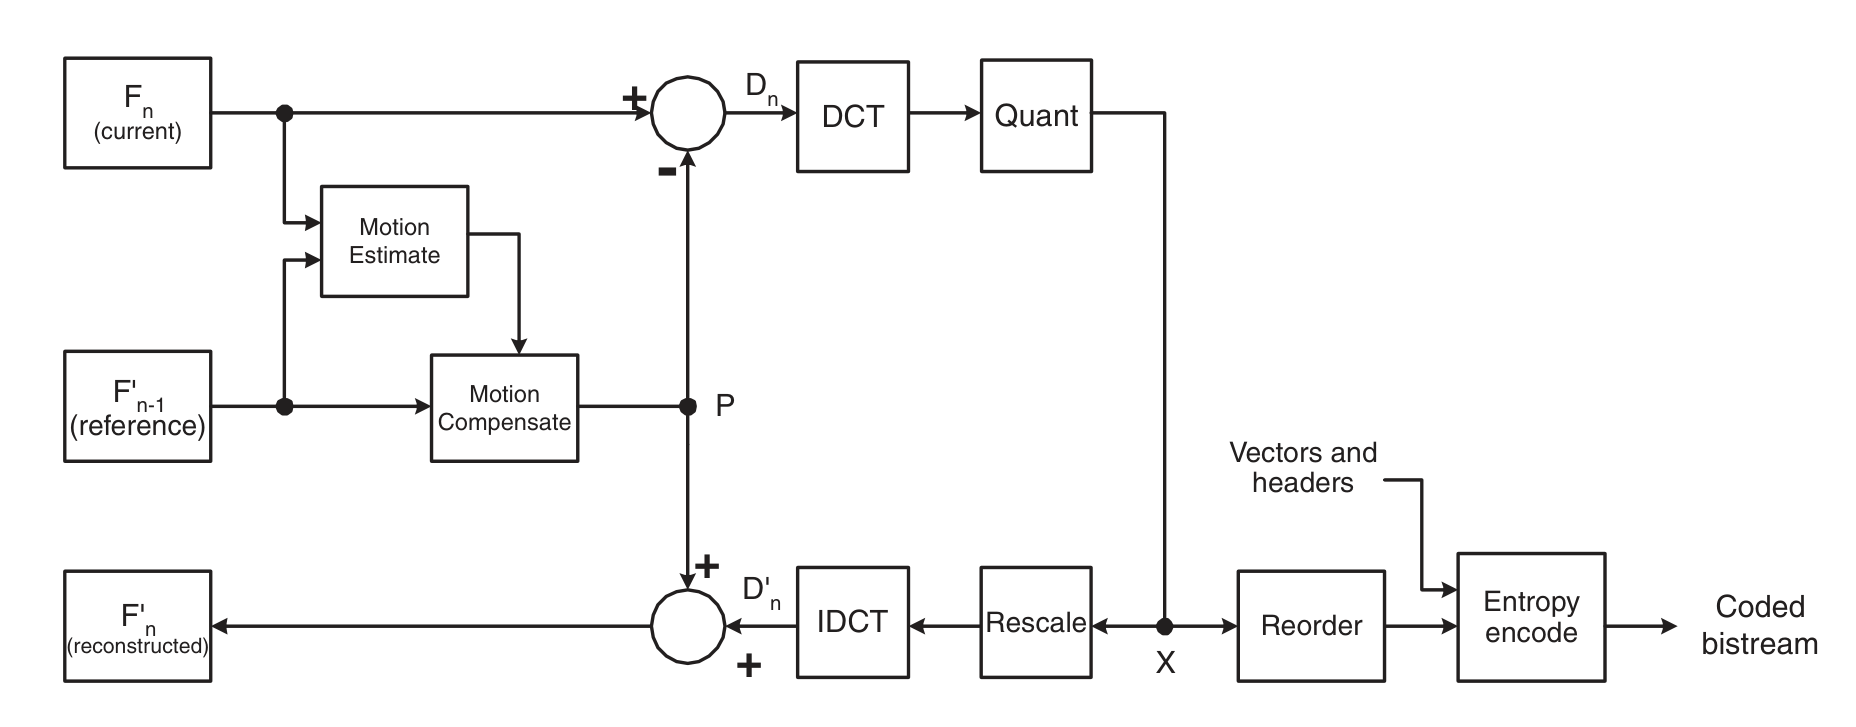
\includegraphics[width=\textwidth]{res/hybrid_codec_detailed.png}
	
	\caption{Detailed hybrid codec architecture.\cite{h264}}
	\label{fig:codec_highlevel}
\end{figure}

%The transform converts the samples into another domain in which they are represented by transform coefficients. The coefficients are quantized to remove insignificant values, leaving a small number of significant coefficients that provide a more compact representation of the residual frame. The output of the spatial model is a set of quantized transform coefficients.

%The parameters of the prediction model, i.e. intra prediction mode(s) or inter prediction mode(s) and motion vectors, and the spatial model, i.e. coefficients, are compressed by the entropy encoder. This removes statistical redundancy in the data, for example representing commonly occurring vectors and coefficients by short binary codes. The entropy encoder produces a compressed bit stream or file that may be transmitted and/or stored. A compressed sequence consists of coded prediction parameters, coded residual coefficients and header information. The video decoder reconstructs a video frame from the compressed bit stream. The coefficients and prediction parameters are decoded by an entropy decoder after which the spatial model is decoded to reconstruct a version of the residual frame. The decoder uses the prediction parameters, together with previously decoded image pixels, to create a prediction of the current frame and the frame itself is reconstructed by adding the residual frame to this prediction.

The output of a hybrid video encoder is a \textit{bit stream} (or \textit{bitstream}), i.e. a compressed sequence of coded residual coefficients and other parameters. The decoder applies the same process inversely in order to reconstruct the original video frames, with some approximation.

\subsection{Frame types and GOP}
\label{sec:bg/compression/gop}

As we have seen, the prediction model can be based on temporal (inter-frame) prediction or spatial (intra-frame) prediction. The type of prediction that is used and which reference frames are used for the prediction determine the type of frame. In particular:

\begin{itemize}
    \item \textbf{I-frames} (\textit{Intra-frames}) are frames that do not require any other frames to be decoded and are thus compressed only through intra-frame prediction.
    \item \textbf{P-frames} (\textit{Predicted frames}) are frames that can reference other previous frames when performing temporal prediction. Depending on the codec, a frame can reference one or more previous frames.
    \item \textbf{B-frames} (\textit{Bi-directional predicted frames}) are frames that can reference both previous and future frames as reference frames in temporal prediction. They are more computationally expensive to encode, but are usually the most compressible ones.
\end{itemize}

Because of inter-frame dependencies, the display order of frames is very often different from the decoding order.

Depending on the type of frames that are used to encode a video sequence, different \textbf{prediction structures} can be obtained. For example, low delay applications could use a structure like the one in figure \ref{fig:codec_gop1}, where only I-frames and P-frames are used and P-frames always reference the previous frame. I-frames need to be inserted in the stream every now and then to allow more efficient random access (\textit{seeking}). Another reason is that in some cases scene cuts might justify the use of an I-frame instead of a P-frame, depending on how drastic the scene change is.

\begin{figure}
	\centering
	
	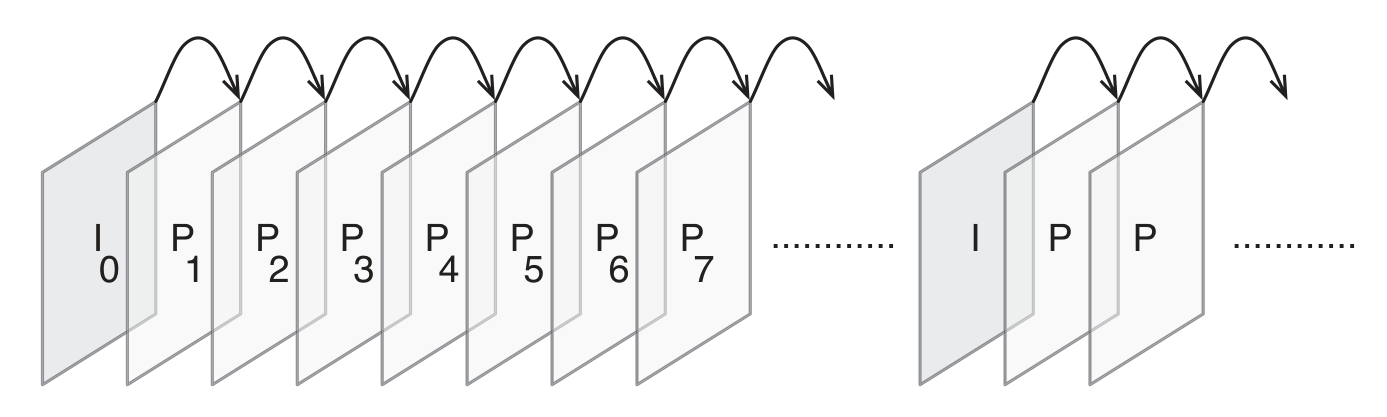
\includegraphics[width=0.9\textwidth]{res/gop1.png}
	
	\caption{Simple GOP structure with no B-frames.}
	\label{fig:codec_gop1}
\end{figure}

Most of the time, the arrangement of the frames is much more complex and is usually defined by a \textbf{Group of Pictures (GOP)} structure, as seen in Figure \ref{fig:codec_gop2}. A GOP always starts with an I-frame and is most of the time \textit{closed}, which means that it is independent from previous and future GOPs. As a consequence, in a closed-GOP scenario the decoder does not need access to previous of future GOPs to be able to decode frames in the current GOP.

The structure of a GOP can be summarized as a string sequence, like \texttt{IBBPBBPBBPBBI}, or through two numbers, \texttt{M} and \texttt{N}, that respectively determine the distance between P-frames, and the GOP size. For example, the structure in Figure \ref{fig:codec_gop2} can be expressed as \texttt{M=3, N=12}.

\begin{figure}
	\centering
	
	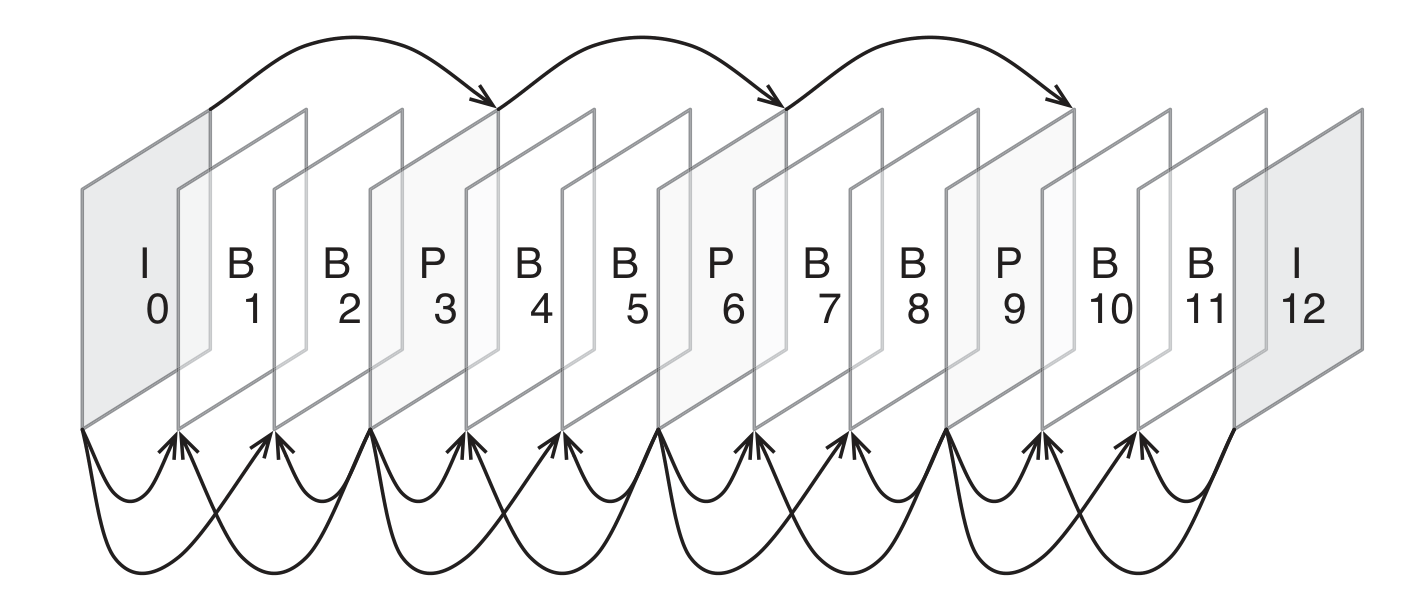
\includegraphics[width=0.8\textwidth]{res/gop2.png}
	
	\caption{Typical GOP structure, \texttt{M=3, N=12}.}
	\label{fig:codec_gop2}
\end{figure}

\subsection{Popular video coding formats}
\label{sec:bg/compression/codecs}

The dominant video coding standard is currently \textbf{H.264}, sometimes referred to as \textit{Advanced Video Coding} (AVC) or \textit{MPEG-4 Part 10}, developed by a joint team of the ITU (Video Coding Experts Group) and ISO (Moving Picture Experts Group, or \textbf{MPEG}). H.264 was first standardized in 2003, nevertheless it is estimated that H.264 is still used today by more than 80\% of the companies in the industry, thanks to its good performance (both in terms of compression and encoding/decoding efficiency) and the accessible royalties structure.\cite{bitmovin}

It is worth noting that the H.264 standard only defines the format and syntax of the H.264 bitstream and how to decode it, but it does not specify how to actually encode a video. This is why the term \textit{codec} should be only used to refer to the actual software implementations of H.264, which typically include both an encoder and a decoder.

The successor of H.264, first published in 2013, is \textbf{H.265}, also named \textit{High Efficiency Video Coding} (HEVC) or \textit{MPEG-H Part 2}, delivering 25\% to 50\% better compression at the same bitrate when compared to H.264. It is especially suitable for high-resolution content like 4K UHD, but it struggled to reach wide adoption because of the complex and expensive royalties structure that slowed down hardware support.\cite{hevcroyalties}

Apart from the H.26x family of formats, Google released the royalty-free \textbf{VP8} in 2008, followed by \textbf{VP9} in 2012. Thanks to Google controlling a large fraction of the browsers market share and the YouTube streaming platform, VP9 became a popular alternative to H.264 often delivering better video compression ratios with comparable quality.

% TODO: sources

The successor to VP9 was incorporated into \textbf{AV1} (first released in 2018), the royalty-free video format developed by the \textit{Alliance for Open Media} (AOMedia), an initiative backed by large companies like Google, Apple, Meta, Microsoft, Amazon, Netflix, Cisco, NVIDIA, Intel, among others.\footnote{\url{https://aomedia.org/membership/members/}} AV1 is much more complex than H.264 and achieves up to 50\% better compression when compared to H.265, making it especially suitable for high-resolution content like 4K UHD or 8K UHD. The downside of AV1 is that since it is quite complex codec implementations are often prohibitively expensive to be run in software, thus requiring hardware support, an effort that can require quite a few years.

% TODO: sources

\subsubsection{H.264}
\label{sec:bg/compression/codecs/h264}

\begin{figure}
	\centering
	
	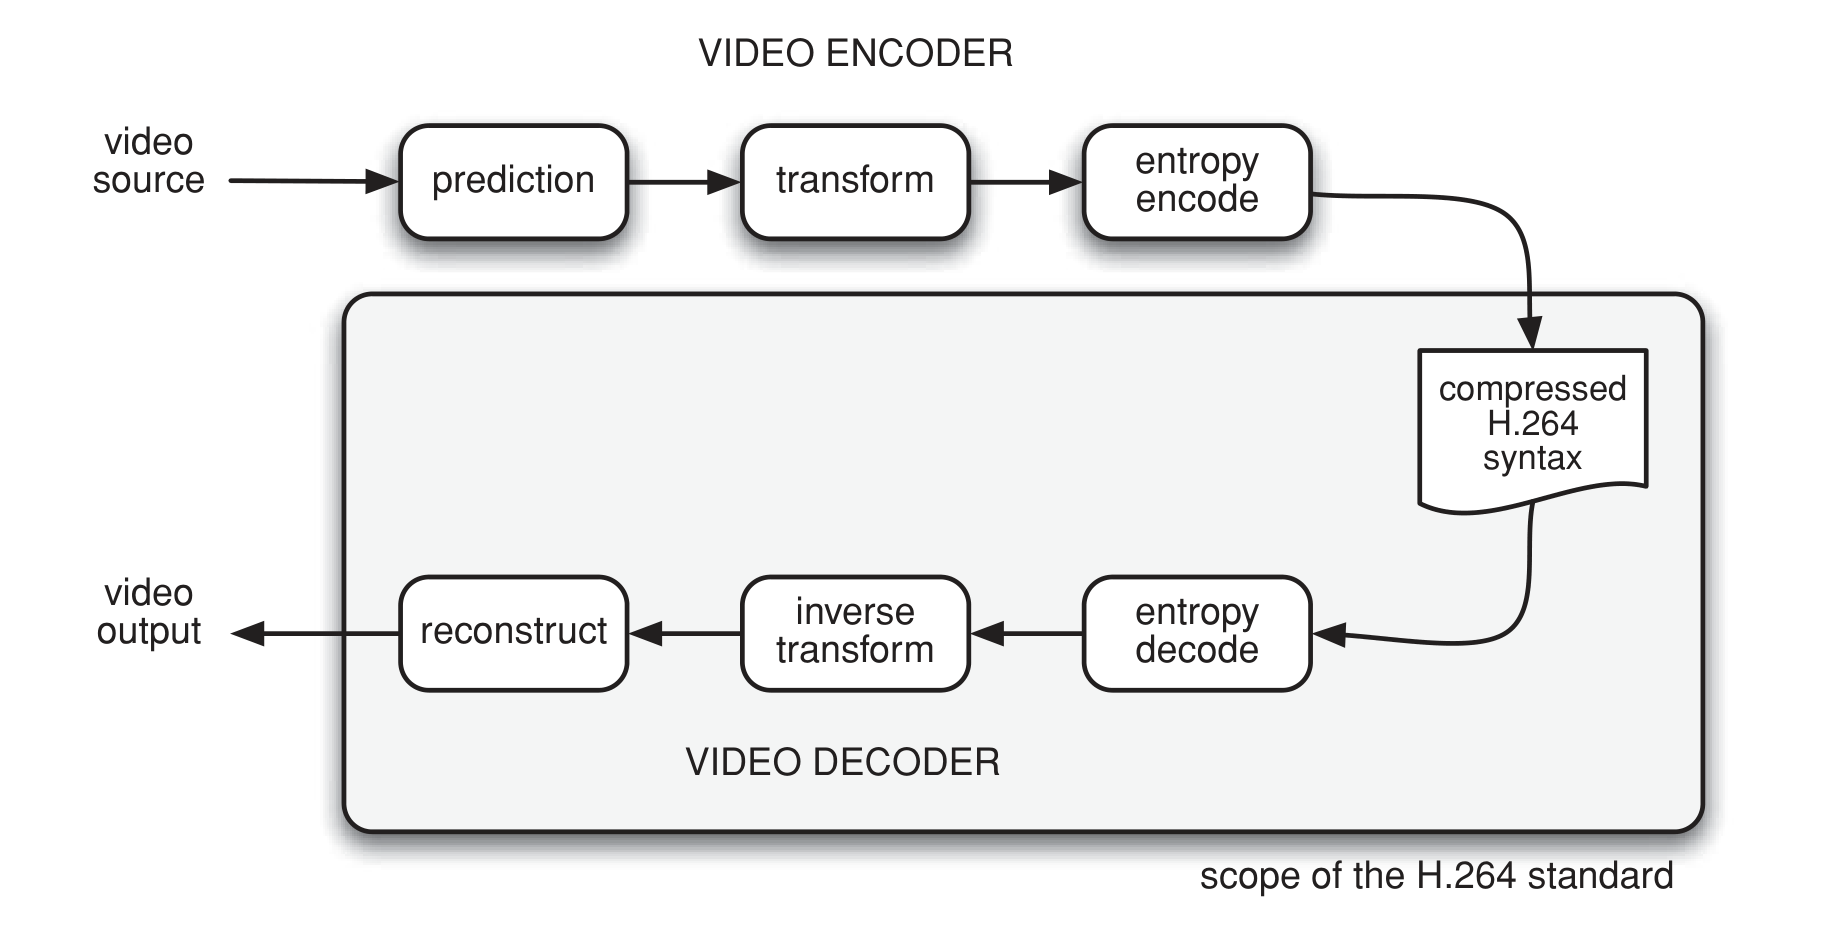
\includegraphics[width=0.8\textwidth]{res/h264_scope.png}
	
	\caption{The scope of the H.264 standard.}
	\label{fig:h264_scope}
\end{figure}

As we have seen, H.264 is still the dominant video format in the industry. Since the standard only covers the decoding part of the codec, as shown in Figure \ref{fig:h264_scope}, many codec implementations have been released, achieving different compression results. One of the most popular H.264 encoders is \texttt{x264}, which is open-source and software-based, typically scoring as the best speed/quality trade-off in H.264 codecs comparisons.\cite{msu2021}

H.264 is based on the hybrid codec model we have introduced above. Frames are divided into 16x16 pixels \textbf{macroblocks} (MB), on which the prediction model is applied. Macroblocks can be split into partitions that can be as small as 4x4 pixels (not necessarily square), so that the same macroblock can reference different macroblocks possibly in different reference frames.

In H.264, the transform is an approximation of the DCT and can be applied on 4x4 or 8x8 blocks. Quantization can be controlled by the QP parameter, or step size, which ranges from 0 to 51 and is usually adjusted automatically by the encoded depending on the input configuration. Finally, for the entropy coding step, H.264 supports both the variable-length coding and arithmetic coding techniques.

As not every device is capable of supporting all the features of the standard, H.264 includes the concept of profiles and levels. A \textbf{profile} defines which H.264 features the decoder must support in order to be able to decode the compressed video. Common profiles are: the baseline profile, which does not include support for B-slices\footnote{In H.264 the concept of I-frames, P-frames and B-frames is replaced by the slices equivalent. A slice is a subset of macroblocks contained in a video frame.} or CABAC\footnote{Context-aware Arithmetic Coding.}; the main profile, which supports both B-slices and CABAC; the high profile, which includes additional optimizations like adaptive selection of the block size for the transform step. The \textbf{level} instead specifies an upper limit on the frame size, decoding rate and memory required to decode the a video.

Finally, an important part of H.264 is the syntax of the coded bitstream. The H.264 data is organized in a sequence of packets known as \textbf{Network Abstraction Layer Units} (NAL units or \textbf{NALUs}). Since the units can be of varying length, there should be a way to distinguish when a unit ends and the next one begins. There are mainly two approaches to solve this problem:

\begin{itemize}
    \item Transporting NAL units into \textbf{packets}, which could be network packets or a structure defined by the \textbf{container format}, as we will see in the following sections.
    \item Treating the bitstream as a \textbf{byte stream}. In this case a \textit{start code}, a 3-byte sequence acting as a synchronization marker, is inserted before each NAL unit so that the decoder can identify the units boundaries. This byte stream format is defined by the \textit{Annex B} of the standard, which is the reason why this format is very often referred to as \texttt{annexb}.
\end{itemize}

\begin{figure}
	\centering
	
	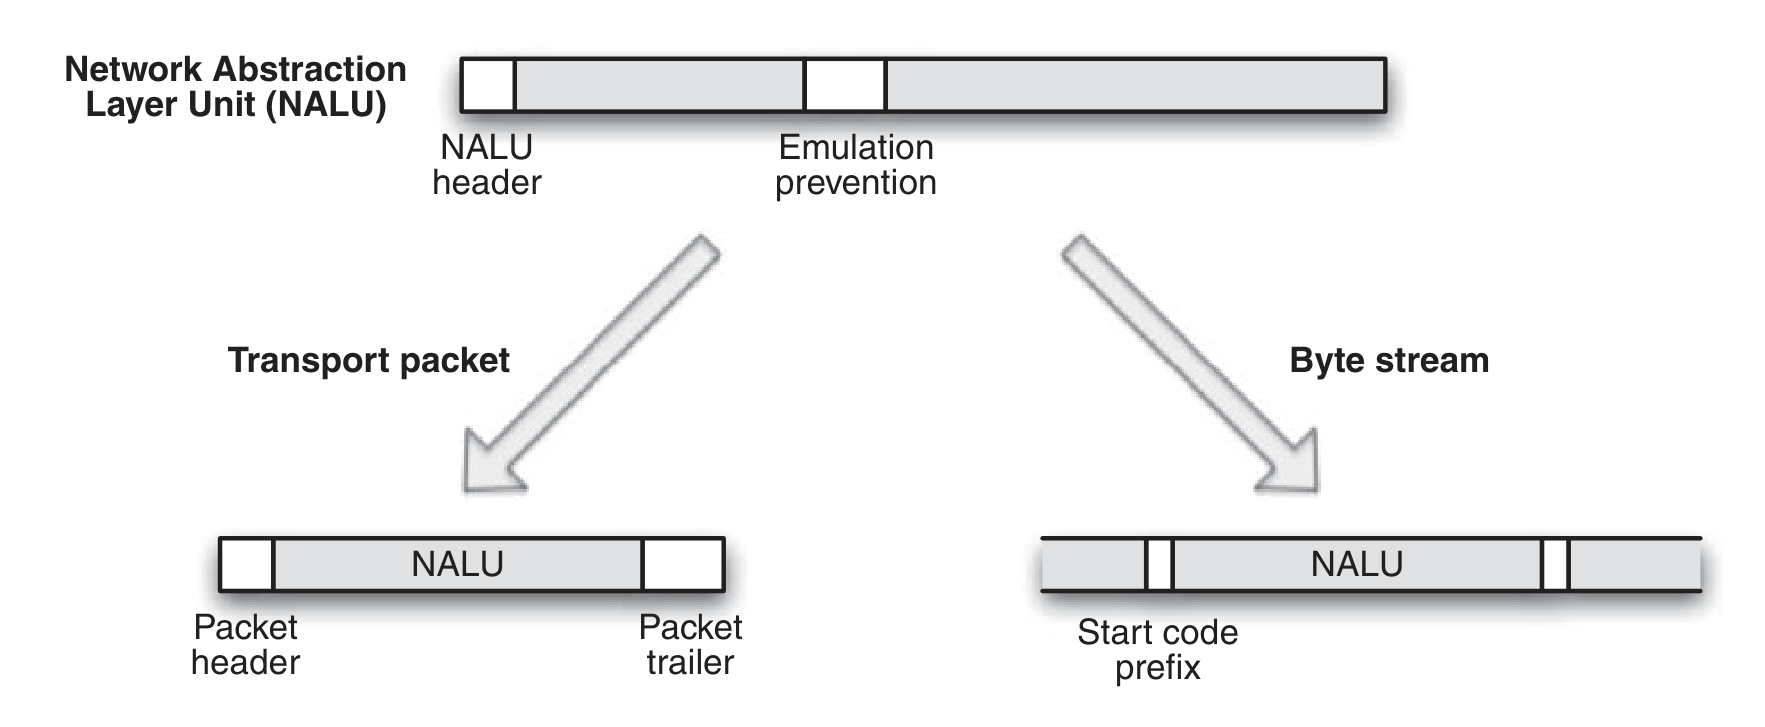
\includegraphics[width=0.9\textwidth]{res/h264_nalu.png}
	
	\caption{H.264 bitstream structure and encapsulation alternatives.}
	\label{fig:h264_scope}
\end{figure}

\section{Digital audio and compression}
\label{sec:bg/audio}

Digital audio is usually represented through the \textbf{Pulse Code Modulation} (PCM) method, which is characterized by two main parameters: the \textbf{sample rate}, defining how frequently the sound level was measured when captured from the analog domain, and \textbf{bit depth}, which refers to the number of bits used to store a sample.

Although uncompressed PCM audio is more tractable than video, since it is much lighter (a stereo audio track with 44.1 kHz sample rate and 16-bit samples requires "only" 1.4 Mbps), audio is typically highly compressible since human sound perception is limited. Audio coding formats such as \textbf{MP3} and \textbf{AAC} are based on perceptual coding, since they tend to discard sound information that would otherwise be inaudible and can achieve excellent quality with savings of up to 90\%.\cite{aac}

\textbf{AAC} is nowadays the most used audio format in streaming scenarios, and is supported by virtually every device.\cite{bitmovin} AAC comes in multiple variants, with \textbf{Low Complexity} (AAC-LC) being the most common since it is widely supported and provides good compression ratios and quality. Other common versions are the ones of the \textbf{High Efficiency} (HE) family, which are optimized for low-bitrate applications.

In the AAC bitstream, audio samples are organized in packets that contain a fixed number of samples, typically 1024. To reduce compression artifacts, AAC uses a modified version of the DCT transform that works with overlapping samples. This means that in practice, for each AAC packet encoded or decoded another packet with the same number of samples is required. For this reason, AAC encoders add at least 1024 samples of silence before the first actual audio sample, a technique called \textbf{priming}. Since this delay could introduce synchronization issues when audio is combined with video, decoders need to detect priming and correctly take into account the encoder delay.\cite{aacpriming}

\section{Container formats}
\label{sec:bg/containers}

Bitstreams produced by video and audio encoders often do not contain enough information to allow video players to actually play the video or audio file. For example, in H.264 the timing information is optional and without it the decoder does not know how to assign timestamps to individual video frames, or even determine the duration of the video.\cite{h264itu} In AAC, the raw frames do not contain information like the sample rate or even the variant of AAC used to encode the samples.\cite{aac}

\textbf{Container formats} solve this problem by wrapping the bitstreams in a structure that is common between different coding formats. Container formats also allow the grouping of multiple video, audio, and subtitle tracks, an operation known as \textbf{muxing} (from \textit{multiplexing}) and performed by \textbf{muxers}. The process of extracting tracks from a container format is instead known as \textbf{demuxing}.

Two popular container formats used in the context of video streaming are \textbf{MPEG-2 Transport Stream} and \textbf{MP4}.

\subsection{MPEG-2 Transport Stream}
\label{sec:bg/containers/mpeg2ts}

MPEG-2 Transport Stream (or \textbf{MPEG-2 TS}), defined by the MPEG-2 Part 1 standard, is a container format originally designed for digital television broadcasting systems. For this reason, it includes features like error correction and synchronization, providing protection from degraded transmission channels.

A single MPEG-2 Transport Stream can transport multiple programs, for example multiple TV channels. Each program can consist of multiple video and audio streams, known as \textbf{elementary streams}. The coded data for each elementary stream is packetized into PES (Packetized Elementary Stream) packets, each having a fixed length of 188 bytes. The 188 bytes include headers (which transport data like timing information), which is the reason why Transport Stream often has a non-negligible overhead.\cite{mpeg2ts}

% terrible, rewrite
% https://tsduck.io/download/docs/mpegts-introduction.pdf

An H.264 bitstream muxed in an MPEG-2 stream must be in the Annex B format with start codes.

\subsection{MP4 and fragmented MP4}
\label{sec:bg/containers/mp4}

MP4 is a container file format based on the \textbf{ISO Base Media File Format} (ISOBMFF). It was extended from Apple's QuickTime File Format (\texttt{.mov}) and first published in 2001 as MPEG-4 Part 14.\footnote{The actual box structure is defined in MPEG-4 Part 12 (ISOBMFF).}\cite{mpeg4part12}

In the \textbf{ISOBMFF} format, the video and audio bitstreams, such as an H.264-compressed video, are stored as tracks and organized in a \textbf{box structure}. The MP4 format is capable of storing metadata like the video duration and per-frame display and decoding timestamps, dealing with issues like synchronization between tracks and random access (\textit{seeking}) of the media file.

% Video and audio frames are usually interleaved, although it is possible to generate "flat" MP4 files where tracks are organized sequentially.

Some ISOBMFF box (or atom) types that are particularly relevant are:

\begin{itemize}
    \item \texttt{ftyp} (\textit{file type}), which includes some general information about the file type, e.g. the version of the MP4 (or QuickTime) specification the file is compliant against.
    \item \texttt{moov} (\textit{movie header}), containing metadata about the tracks, such as the creation time, the duration, the resolution, bitrate, the tables that allow players to quickly find the part of the file where a specific frame or timestamp can be found, etc.
    \item \texttt{mdat} (\textit{movie data}), containing the actual audio and video samples.
\end{itemize}

An H.264 bitstream muxed in an MP4 container does not need start codes and therefore must not be in the Annex B format. H.264 bistreams in MP4 files are stored in a format known as \texttt{avcC}, where H.264 NAL units are prepended with their length.

A typical structure of an MP4 file consists of a \texttt{ftyp} box followed by a \texttt{moov} box (containing the tracks metadata), and finally the actual data stored in a \texttt{mdat} box. The \texttt{moov} box is sometimes placed at the end of the file, since the data contained in it is often available only at the end of the encoding process.

% TODO: mp4dump example

For some use cases, like adaptive video streaming, a more suitable structure is the one provided by the \textbf{fragmented MP4} format, or \textbf{fMP4}. In this format, the sequence is divided in fragments that can be transmitted and played independently. The structure of a fMP4 file still has \texttt{ftyp} and \texttt{moov} boxes at the beginning, shared among all the fragments, while the rest of the file consists of a sequence of \texttt{moof} and \texttt{mdat} boxes, where the \texttt{moof} box contains metadata about the fragment, like the fragment index and the timestamp, and the \texttt{mdat} contains the video or audio samples for a single fragment (typically a few seconds of content).

% TODO: mp4dump example

\section{A typical live streaming architecture}
\label{sec:bg/compression}

In a live streaming architecture, we can generally distinguish three main parts: \textbf{ingestion}, \textbf{transcoding and packaging}, and \textbf{distribution}.

\textbf{Ingestion} refers to the process of making the input feed available to the transcoder server for processing. Often, this means having a client push the stream through an ingestion protocol such as \textbf{Real Time Messaging Protocol} (RTMP). In some cases, a more suitable approach is a pull-based one, where it is the backend system's responsibility to "pull" the video and audio streams from another system and pass them onto the pipeline.

Usually, the input feed is a high-bitrate/high-quality stream that is not suitable for live streaming. In particular, when the setup is based on adaptive bitrate streaming (ABR), which is the de facto standard for live streaming, the video stream must be \textbf{transcoded} in multiple video renditions with different quality levels and encoding parameters. The video and audio files produced by this step need to be in a coding and container format that is compatible with the adaptive bitrate technology that was chosen. For example, MPEG-DASH (see Section \ref{sec:bg/technologies/dash}) requires streams to be muxed in a fragmented MP4 container.

Ideally, for the best performance, the video files produced in this step should take into account how ABR technologies work. For example, the bitrate of the individual renditions should not oscillate too much so that bitrate adaption algorithms can take the average bitrate as a reference value. Also, since segments should be roughly of the same size a fixed GOP size should be used when encoding.\cite{ozer}

Additionally, some adaptive streaming technologies require the video fragments (or segments) to be stored in physically separated files. The task of splitting video and audio files into smaller segments is done by \textbf{packagers}, which can be static or dynamic: with \textbf{static packaging} the individual video fragment files are actually created and stored on disk, while with \textbf{dynamic packaging} they are generated on the fly. The packager, which is specific for the ABR technology, also creates \textbf{manifest or playlist files} that act as an index for the streams.

The segmented video and audio tracks, together with the manifest files, can finally be delivered to clients. Most of the time, this is done through the Hypertext Transfer Protocol (HTTP). Using HTTP makes it easy for streaming platforms to scale, thanks to the widespread availability of \textbf{Content Delivery Networks} (CDN) and their global distribution networks. One of the important advantages of relying on CDNs is the possibility to cache video segments at the edge of the networks, as close as possible to the final users, therefore reducing latency and probability of congestion.

% architecture diagram

% TODO: probably merge this section with the below one and be more precise with terminology. See NMD report.

% TODO: packager or segmenter

% advantages of HTTP: no UDP, firewalls, scalability, https

\section{Adaptive bitrate technologies}
\label{sec:bg/abr}

\subsection{Apple HTTP Live Streaming (HLS)}
\label{sec:bg/abr/hls}

HTTP Live Streaming (HLS) is an HTTP-based adaptive streaming protocol designed by Apple. First introduced in 2009 and later standardized as RFC 9216, it is estimated to be the most popular streaming protocol with over 73\% companies using it.\cite{rfc8216}\cite{bitmovin} The reason for that is not only the fact that HLS is the only possible option to implement live and on-demand streaming on Apple mobile devices and browsers, but also the simplicity of the protocol.

HLS uses the \textbf{extended M3U format} (\texttt{.m3u8} extension) to define a set of playlists, containing information such as the list of streams or the list of segments for a particular stream. In particular, a \textbf{master playlist} provides a set of variant streams\footnote{In the HLS RFC, the terms \textit{variant} and \textit{rendition} have different meanings. We will use the term \textit{variant} in this section to adhere to the RFC, while using the two terms interchangeably in the rest of the thesis.}, each of which is a different version of the same content, usually differing by the bitrate and other encoding parameters. Players download the master playlist at the beginning of the playback session and use the information contained in it to adapt to network conditions by switching between variants. An example of a master playlist is shown in Figure X.

% TODO: master playlist example

When players want to play a specific variant, they load the \textbf{media playlist} corresponding to the variant. A media playlist must specify the maximum duration of segments in seconds, followed by a list of \textbf{media segments}, characterized by their duration and URI (relative or absolute). In the case of an on-demand content, the media playlist must contain the full list of segments that make the video or audio file, while in the case of live streams the playlist may include only a sliding window of segments. An example of a media playlist is shown in Figure Y.

Media segments in HLS can be muxed in the MPEG-2 TS format (\texttt{.ts} files) or fragmented MP4 (\texttt{.mp4} or \texttt{.m4s} files), while the supported video codecs are H.264 and H.265. When using \texttt{fMP4} as a container format, media playlists must specify an \textbf{initialization segment} containing the \texttt{ftyp} and \texttt{moov} boxes through the \texttt{\#EXT-X-MAP} tag.

In addition to the RFC, Apple maintains an \textit{Authoring Specification for Apple Devices} defining additional rules for HLS streams which are often taken as best practices in the industry when producing content for adaptive bitrate streaming.

The authoring specification provides a set of recommendations to ensure compatibility with HLS implementation that can be found on Apple devices, including:

\begin{itemize}
    \item a table with a possible set of variants with their bitrate and frame rate (a \textit{bitrate ladder}), for both H.264 and H.265, plus a recommendation to adjust them according to the specific use case;
    \item an indication that the peak bitrate should be no more than 200\% of the average bitrate, although it is often recommended to make the bitrate as constant as possible;\cite{ozer}
    \item a recommendation for a segment duration of 6 seconds, although 4 seconds or lower are common values in practice.\cite{ozer}
\end{itemize}

HLS also includes support for encryption, ads, trick play (scrubbing and fast forward), subtitles, and multiple audio tracks.

% TODO: low-latency HLS

\subsection{MPEG Dynamic Adaptive Streaming over HTTP (DASH)}
\label{sec:bg/technologies/dash}

% TODO

\subsection{Common Media Application Format (CMAF)}
\label{sec:bg/technologies/cmaf}

Before Apple introduced support for \texttt{fMP4} in 2016, a common issue for video platforms was that supporting both HLS and DASH required to maintain two copies of the same content, one in MPEG-2 TS format and the other one in \texttt{fMP4}.

This led to the proposal and standardization of the \textbf{Common Media Application Format} (CMAF), a common specification that defines how media should be packaged and segmented for delivery. Fragmented MP4 is a CMAF-compatible format and since it is supported by both HLS and DASH it can lead to significant savings. Video platforms can in fact produce and store a single set of video segment files which can be delivered to all devices.\cite{cmaf}

\subsection{Media Source Extensions (MSE)}
\label{sec:bg/technologies/mse}

One of the main medium through which users watch video streams is web browsers. Apple includes native support for its HLS protocol in Safari, which is pre-installed on all Apple devices and is also the only engine that can be used on iOS. Other browser typically do not include support neither for HLS or DASH, but instead support the \textbf{Media Source Extensions} (MSE) API, through which JavaScript libraries can implement support for HLS and DASH.\cite{mse}

MSE is a set of APIs that abstract the implementation of media playback in the browser. MSE exposes types and methods that allow the client-side code to push video and audio data for playback.

More in detail, MSE defines the \texttt{MediaSource} type as a source of media data for the \texttt{<video>} or \texttt{<audio>} HTML5 media elements, to which a \texttt{MediaSource} is attached. The client code interacts with the \texttt{MediaSource} to push new data while media elements fetch the data from the \texttt{MediaSource}.

\texttt{MediaSource} instances expose methods to attach a set of \texttt{SourceBuffer} objects, which represent individual media tracks like a video or audio streams. When new media data is available, such as a new video segments, the client calls the \texttt{appendBuffer()} method on the corresponding \texttt{SourceBuffer}, providing the new data for the track to the browser. The bytes of data must of course conform to the format set when creating the \texttt{SourceBuffer}, which must be supported by the browser. Most of the time this means ISOBMFF (\texttt{fMP4}) or WebM as container formats, while codecs often depend on the browser build and platform.

Libraries that implement HLS or DASH must take care of parsing the manifest files, downloading the segments, implementing rate adaption algorithms, potentially transmuxing from MPEG-2 TS to fragmented MP4 (such as with HLS), appending segment data to the source buffers while leaving the MP4 demuxing and stream decoding tasks to the browser.

In practice, this means that there can be many implementations of HLS and DASH, all relying on Media Source Extensions underneath. For HLS, a popular implementation is \texttt{HLS.js}\footnote{\url{https://github.com/video-dev/hls.js/}}, while for DASH the official reference implementation is \texttt{dash.js}\footnote{\url{https://github.com/Dash-Industry-Forum/dash.js/}}. Several other JavaScript players include support for HLS and DASH, such as \texttt{Video.js}, \texttt{Shaka Player}, \texttt{THEOPlayer}, and \texttt{JW Player}, some of which are open source while other are commercial.

\section{Hypertext Transfer Protocol (HTTP) evolution}
\label{sec:bg/http}

\subsection{HTTP/1.1}
\label{sec:bg/http1}

\subsection{HTTP/2}
\label{sec:bg/http2}

\subsection{HTTP/3}
\label{sec:bg/http3}

\section{Network emulation tools}
